\chapter{The Problem of Being Inside the System}


\section{The Internal Perspective}

Physics has a fundamental problem: we are trying to describe a system from the inside.

At least, it certainly appears that way. The universe is vast; we are small. In the language of set theory, we are the subset O attempting to map the superset U.

\begin{figure}[h]
    \centering
    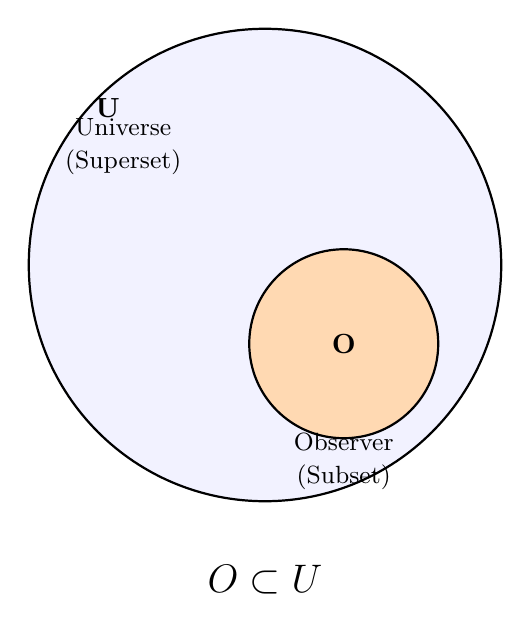
\begin{tikzpicture}
        % The Universe U
        \draw[thick, fill=blue!5] (0,0) circle (3cm);
        \node at (-2,2) {\textbf{U}};
        \node[text width=2cm, align=center] at (-1.8,1.5) {\small Universe\\(Superset)};

        % The Observer O
        \draw[thick, fill=orange!30] (1,-1) circle (1.2cm);
        \node at (1,-1) {\textbf{O}};
        \node[text width=2cm, align=center] at (1,-2.5) {\small Observer\\(Subset)};

        % The Notation
        \node at (0,-4) {\Large $O \subset U$};
    \end{tikzpicture}
    \caption{The problem of internal perspective: $O$ is a subset of $U$.}
\end{figure}


Because we are embedded, we cannot help but see through a human lens. We experience "time" as a flow and "matter" as solid objects, but these might simply be illusion of our perspective.
This makes it incredibly difficult to distinguish between a fundamental law of nature and a mere byproduct of our vantage point. We are not external spectators; we are looking at the machine while our own bodies are being ground between its gears.

This feels "right." Intuitively, we want to believe that the majestic universe would exist exactly as it is even if we never appeared. It seems arrogant to suggest that our pitifully thin layer of brain matter could play any significant role in the fundamental existence of the cosmos.

But this is the trap. Even if the universe exists without us, the description of it—the physics we write down—is entirely filtered through our internal perspective.
If you are inside a house, you can’t describe the roof without acknowledging you’re looking up from the floor.
By trying to write "God-eye" equations, we have ignored the most important variable: the fact that the person doing the math is part of the equation.

\section{The Method}

We don’t truly know what time is—perhaps because we are submerged within it. But while the essence of time remains elusive, we can simulate it.

If we build a digital universe that duplicates the essential properties of our own, then whatever "mystery" we don’t understand must be present within the machine running the code. The problem of the "Unknown" is suddenly reduced to the "Known."

We may not understand the cosmos, but we understand software completely. By moving the mystery from the vacuum of space into a block of silicon, we turn a metaphysical puzzle into a debuggable program.

